%forklar toolchain skidtet
%regneark med data - parameter til python - til cora model - til cora verifyta - til læsbart trace - til python - til SMC model - til query - til python - til start/til scheule
\section{Tool-chain} \label{sec:tool_chain}
[Før dette læses, så er de diverse tools blevet introduceret. Her er CSV fil formattet også forklaret]\\
\Cref{fig:tool_chain} displays the flowchart representation of the tool-chain. The numbers that are used are only their for the convenience of this section as we will present some of the locations. 

\paragraph{Location 1 - CSV file that contains payload information} is the input file for the system. This usage of this file and its format is described in [INSERT REFERENCE]

\paragraph{Location 2 - Generate CORA XML models file from input} in this location we will read the CSV file or the tuned parameters from location 9. The input is used to generate the two \gls{cora} model. One models uses the worst case values and the other will use the original values. 

%\paragraph{Location 3 - Input model to CORA Verifyta} the Verfyta will generate a trace for each model.

\paragraph{Location 4 - Test worst case model} run the queries for the worst case model.

\paragraph{Location 5 - Is the worst case possible?} if we were unable to produce a trace for the worst case, we will not be able to guarantee that any of the schedules we produce will hold. We will go to location 6, the fail state, if we unable to produce such a trace.

\paragraph{Location 7 - Extract trace from the "normal" model and it to LIBUTAP} [find et andet navn end "normal model"] we will extract, or produce, a trace in this location from the "normal model" and use it as input for the tracer function in LIBUTAP. The tracer function will transform it into a human readable trace.

\paragraph{Location 9 - Convert trace to SMC XML model file} in this location we will read the trace and produce the SMC model that will be used in the next location.

\paragraph{Location 10 - Verify queries and extract the results} 

\begin{figure}
	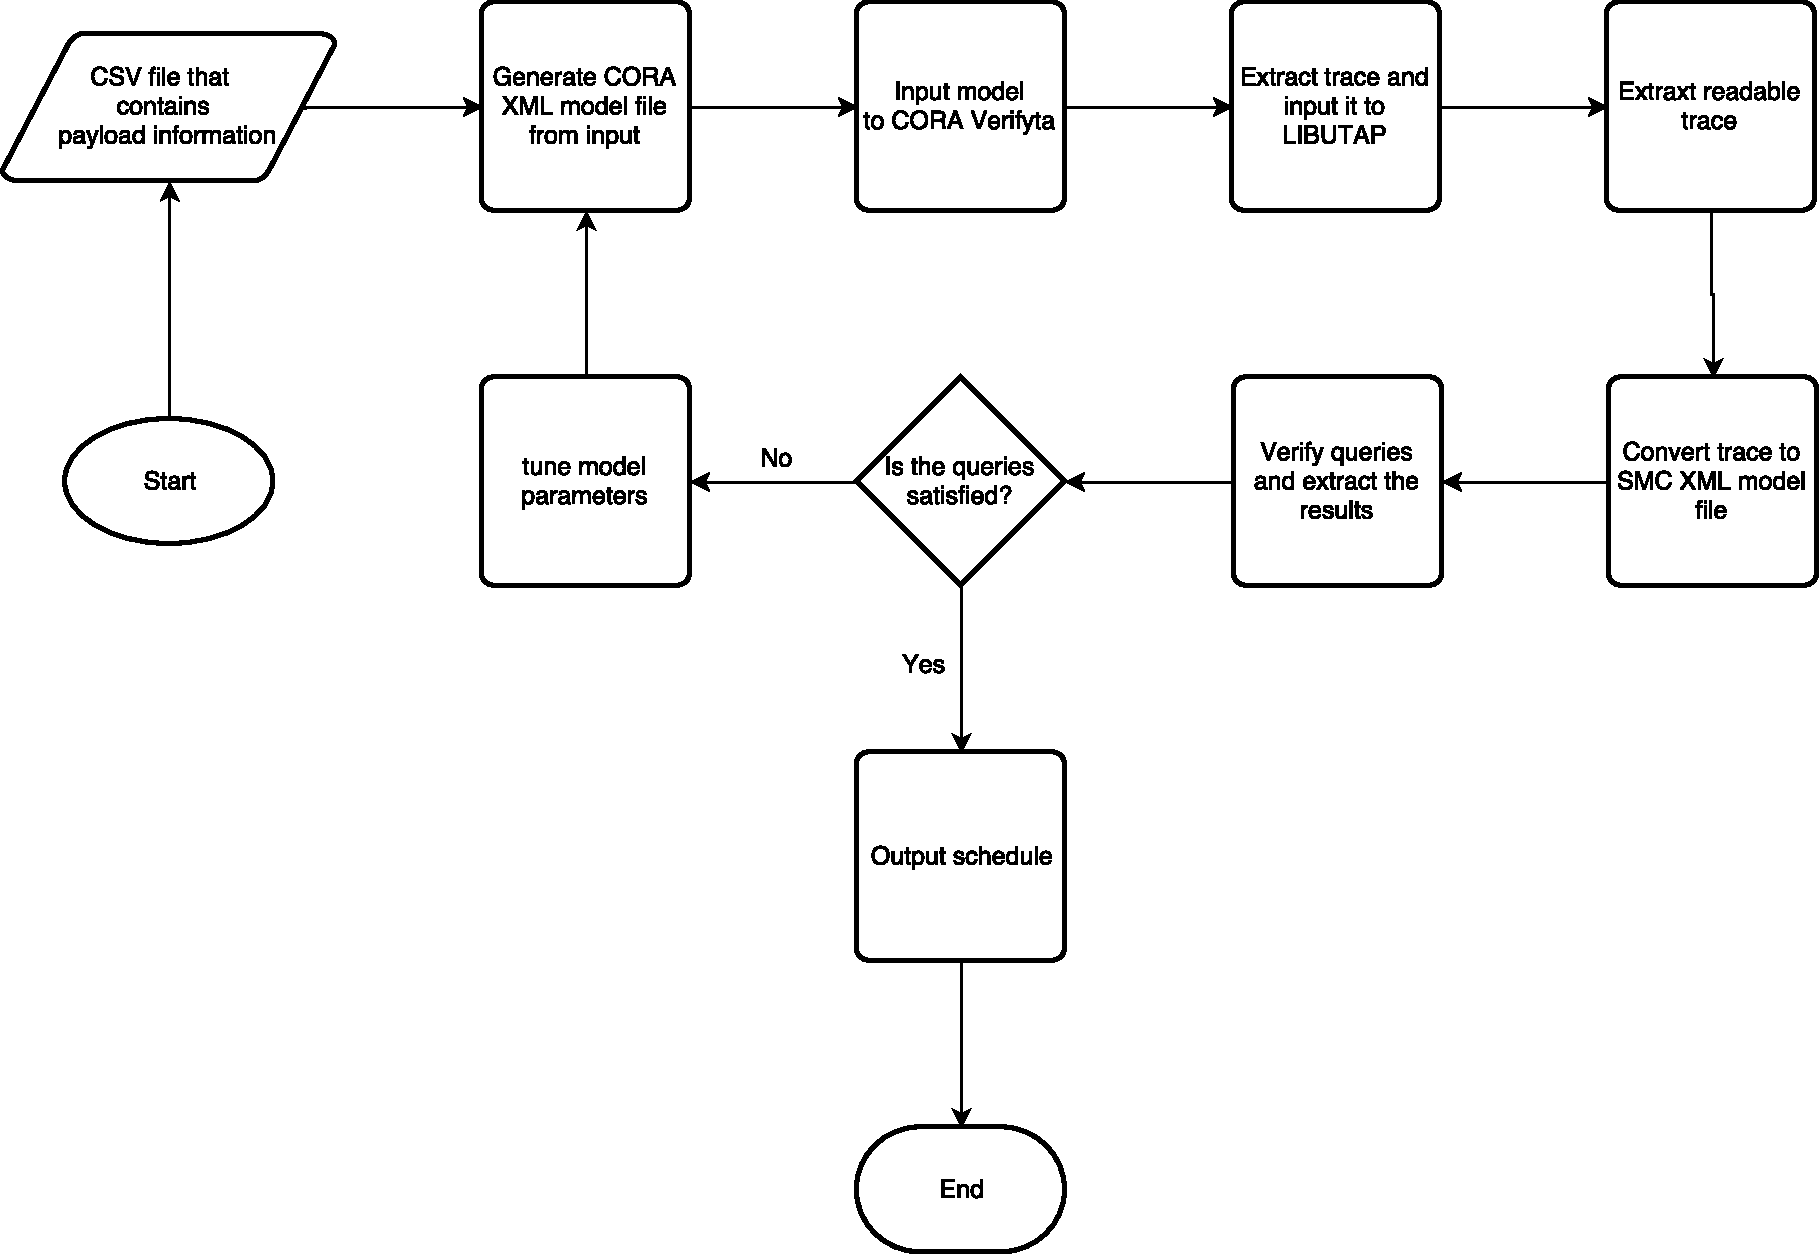
\includegraphics[width=\textwidth]{graphics/tool_chain.pdf}
	\label{fig:tool_chain}
	\caption{My caption}
\end{figure}